\scanpage{74}
% archive sheet number: 73
% @ top left, four directed horizontal strokes and crossing slants
\figure{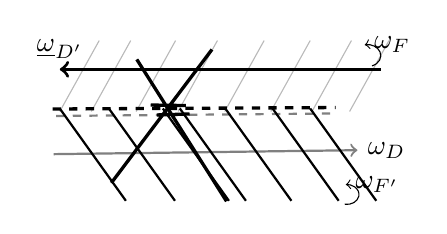
\begin{tikzpicture}[x=.77cm,y=.63cm]
\foreach \x in {0,.52,1.26,1.95,2.72,3.48,4.16,4.78}{\draw[gray!55] (\x,.6)--++(.65,1.43);}
\draw[very thick,<-] (0,1.45) node[above]{$\underline\omega_{D'}$}--(5.3,1.45);
\draw[very thick,dashed] (-.12,.65)--(4.55,.68);\draw[thick,dashed,gray] (-.06,.51)--(4.54,.56);
\draw[gray,thick,->] (-.1,-.26)--(4.91,-.18) node[right,black]{$\omega_D$};
\foreach \x in {0,.81,1.7,1.98,2.73,3.51,4.13}{\draw[thick] (\x,.66)--++(1.09,-1.86);}
\draw[very thick] (1.27,1.65)--(2.75,-1.21) (.85,-.84)--(2.51,1.85) (1.5,.73)--(2.08,.72) (1.6,.53)--(2.14,.55);
\draw[->] (5.15,1.52) arc(-70:102:.22) node[right]{$\omega_F$};
\draw[->] (4.7,-1.27) arc(-100:95:.20) node[right]{$\omega_{F'}$};
\end{tikzpicture}\hspace{.55em}
% @ top middle and right, bracketed alternative
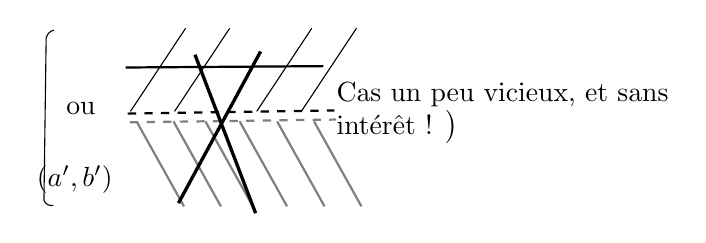
\begin{tikzpicture}[x=.70cm,y=.58cm]
\draw (-1.14,2.1) to[bend right=28](-1.28,1.93)--(-1.32,-1.63) to[bend right=38](-1.15,-1.74);
\node at (-.65,.38){ou};\node at (-.76,-1.18){$(a',b')$};
\draw[thick] (.16,1.28)--(3.75,1.31);\draw[thick,dashed] (.2,.27)--(3.95,.34);\draw[gray,thick,dashed] (.24,.08)--(3.98,.14);
\foreach \x in {.25,1.05,2.54,3.35}{\draw (\x,.32)--++(1,1.82);}
\foreach \x in {.36,1.03,1.61,2.23,2.91,3.58}{\draw[gray,thick] (\x,.1)--++(.86,-1.86);}
\draw[very thick] (1.42,1.56)--(2.52,-1.91) (1.12,-1.69)--(2.61,1.63);
\node[align=left] at (7,.28) {Cas un peu vicieux, et sans\\ intérêt ! $\big)$};
\end{tikzpicture}}

% @ L1–2, heading
\deleted{\unsure{4)|A)}} Cas $(a,b)$ \deleted{c'est le cas} de \uline{prolongation des rives}.

% @ L3–5
1) On choisit comme recollement le transport parallèle. On trouve un $\unsure{\mathscr X|X|\mathcal X}$ avec $\varphi:\mathscr X\to X$ qui est une immersion.

% @ L6–13
Dans $\mathscr X$, on a un graphe top. $K$, et les faces de $(\mathscr X,K)$ correspondent aux pos. stables. \deleted{\unsure{On a un}} On a un $L=\varphi^{-1}(X_1)$, qui matérialise la corr. entre faces et pos. stables -- en remplaçant chaque face $F$ par la face $F^{\sim}$ obtenue en la ``gonflant'' aux pts \deleted{qui} ``critiques'' de $\partial K$ i.e. les pts de $K\cap S(L)$.

% @ R1–7, main text
Partons d'une orientation $\omega=\underline\omega_F$ de $F=\Delta_D^*$, et d'un $\omega_D$ orientation de $D$, passant à l'orientation $\omega'$ de $\Delta_{D'}^*$ déduite par transport i.e. le vrillement, \deleted{\unsure{obte|obtient}} orientation $\omega_{D'}$ de $D'$, on constate encore que c'est l'\uline{opposé} de celle obtenue par transport parallèle !

% @ alongside R1–3 and R6–7
% slanted
\margin{\uline{NB} Ici, on \unsure{dilate|déduit} $\Delta_D^*$ en \unsure{prolongeant|prolg|prolonge} en $\unsure{D'|D|D_i}\cap\Delta_{D'}^*$}

\margin{L'ennui, c'est que les circuits sont \unsure{détestables|détables}. On n'obtient \ensuremath{=} pas les bons circuits supersinguliers !}

% @ R8–15
2) Recollement par l'iso $a\unsure{\simeq|\overset{\sim}{\longrightarrow}}b$ opposé au transport parallèle. Cette fois, c'est au niveau de la transition $\underline\omega_F$ \unsure{---,|---|\ensuremath{\to}} $\underline\omega_{F'}$, interprétée comme $\underline\omega_D$ --- $\underline\omega_{D'}$, qu'on obtient le transport parallèle. Contrairement à ce que je croyais, \inserted{encore hier} on trouve les bons circuits autour des positions supersingulières.
